\documentclass[11pt]{article}

\usepackage[margin=1in]{geometry}
\usepackage{graphicx}
\usepackage{booktabs}
\usepackage{amsmath}
\usepackage{hyperref}
\usepackage{caption}
\usepackage{subcaption}

\graphicspath{{../figures/}{figures/}}

\title{Thayer-Net: Controlled Galaxy Deblending with Direct, Residual, and Balanced Residual U-Net Models}
\author{Thayer-Net Project}
\date{\today}

\begin{document}

\maketitle

\begin{abstract}
We present Thayer-Net, a controlled synthetic benchmark for galaxy deblending
with Galaxy10 DECaLS cutouts. The benchmark constructs foreground-only blends
with known clean targets, avoiding rectangular artifacts from naive cutout
addition. We compare identity and threshold baselines with Thayer-Direct,
Thayer-Residual, and Thayer-BR v0.1. Thayer-Direct improves
affected-region mean squared error over identity on normal held-out blends, but
hard stress testing reveals weaker robustness under stronger overlap and
contaminant conditions. Thayer-Residual improves stress performance by learning
contaminant light to subtract, and Thayer-BR v0.1 further improves both normal
and stress aggregate affected-region error by changing the training
distribution. The results support controlled synthetic
deblending as a useful model-comparison setting, while remaining limited by
simplified sky, PSF, noise, and source-environment assumptions.

\end{abstract}

\section{Introduction}
Galaxy deblending is necessary when overlapping astronomical sources bias
measurements of flux, color, morphology, or downstream redshift inference. Real
survey deblending is difficult because overlapping light can be physically
ambiguous and because imaging conditions introduce sky, PSF, detector, and
crowding effects.

This work focuses on a narrower controlled question: given synthetic blends
with known clean targets, can compact U-Net models recover target galaxies more
accurately than simple baselines, and how does performance change under harder
blend conditions? This controlled setting does not solve survey-grade
deblending, but it makes reconstruction targets known and enables direct
evaluation of model behavior.

The experiments compare a progression of learned formulations. Thayer-Direct
predicts the clean target from the blended image. Thayer-Residual predicts the
contaminant residual layer and reconstructs by subtraction. Thayer-BR v0.1
keeps the residual objective but changes the training distribution toward
normal blends, core-overlap blends, and brightness/size stress blends.
Thayer-BR v0.2 Moderate keeps the same residual family and adds a moderate
affected/core-weighted residual loss. Thayer-BR v0.2 Strong is evaluated as a
loss-weighting ablation.


\section{Data and Synthetic Blend Construction}
The project uses Galaxy10 DECaLS cutouts~\cite{galaxy10decals} stored locally as an HDF5 file. The
dataset is not included in the repository. The historical protocol split HDF5
row indices before blending, but exact duplicate sources still crossed those
partitions. The corrected development protocol groups exact pixel hashes and
exact coordinates before assigning train, validation, or development-test
sources. Both blend roles stay inside their assigned group-disjoint partition.
This fixes the demonstrated exact leakage for grouped development evaluation;
it is not an untouched final-paper split and does not prove exhaustive
near-duplicate identity.

Each synthetic blend starts with a target image and a contaminant image from the
same split. Rather than adding a full rectangular contaminant cutout, the
pipeline estimates and subtracts the contaminant background, extracts central
foreground light, applies halo-aware masking, and adds only the foreground
component to the target. This reduces artificial rectangular boundaries and
double-background artifacts that could make the task easier for the wrong
reason.

The generator records sampled shift, brightness, blur, noise, and size-ratio
metadata. These values are useful provenance metadata, but they are not treated
as final model difficulty labels.


\section{Methods}
The identity baseline returns the blended image unchanged. The threshold
baseline uses simple thresholding and connected-component logic to remove bright
regions. These baselines are intentionally simple references; thresholding can
perform worse than identity because removing bright pixels is not equivalent to
reconstructing hidden target structure.

Thayer-Direct follows the encoder-decoder U-Net design
\cite{ronneberger2015unet} and maps a blended image $X$ to a clean target image
$Y$:
\[
    \hat{Y} = f_{\theta}(X).
\]
The model is a compact encoder-decoder U-Net with skip connections.

Thayer-Residual predicts
\[
    R = X - Y,
\]
and reconstructs the target by subtraction:
\[
    \hat{Y} = X - g_{\theta}(X).
\]
This objective can preserve unchanged target light through the subtraction path.

Thayer-BR v0.1 is not a new architecture; it is a residual U-Net trained on a
more targeted blend distribution: 50\% normal/random blends, 30\%
high-overlap/core-obstruction blends, and 20\% brightness/size stress blends.
This tests whether targeted hard-case sampling improves robustness without
changing the basic model family.

Thayer-BR v0.2 Moderate keeps the residual U-Net formulation and balanced
training distribution target, but changes the loss. It uses a normalized
weighted residual mean squared error:
\[
    \mathcal{L} =
    \frac{\sum_i w_i \left(g_{\theta}(X)_i - (X_i - Y_i)\right)^2}
         {\sum_i w_i}.
\]
The affected mask is computed from the known synthetic pair,
\[
    \mathrm{mean}_c(|X - Y|) > 0.02,
\]
not from model predictions. The moderate setting adds weight to affected pixels
and additional weight to affected target-core pixels. Thayer-BR v0.2 Strong
uses larger affected/core weights and is treated as an ablation.


\section{Evaluation}
Evaluation reports whole-image MSE, MAE, PSNR, and SSIM, along with
affected-region MSE and MAE. Affected-region metrics are primary because most
pixels in each synthetic cutout are unchanged. The affected region is defined by
pixels where the blended image differs from the clean target by more than the
affected threshold after averaging absolute RGB differences.

The hard stress test uses 1,000 blends with maximum shift 18, brightness range
0.8 to 1.4, blur range 0.0 to 0.15, noise range 0.0 to 0.006, rotation off,
minimum size ratio 0.75, minimum affected mask fraction 0.01, and affected
threshold 0.02.

The analysis distinguishes generation difficulty, blend severity, target-core
obstruction, and model failure. Blend severity measures image-level damage, not
model difficulty. Model failure is measured by affected-region model error and
improvement relative to identity.


\section{Results}
Figure~\ref{fig:affected-mse} summarizes the original row-index development
evaluation. These preserved figures are historical context, not the primary
grouped estimate.

\begin{figure}[t]
    \centering
    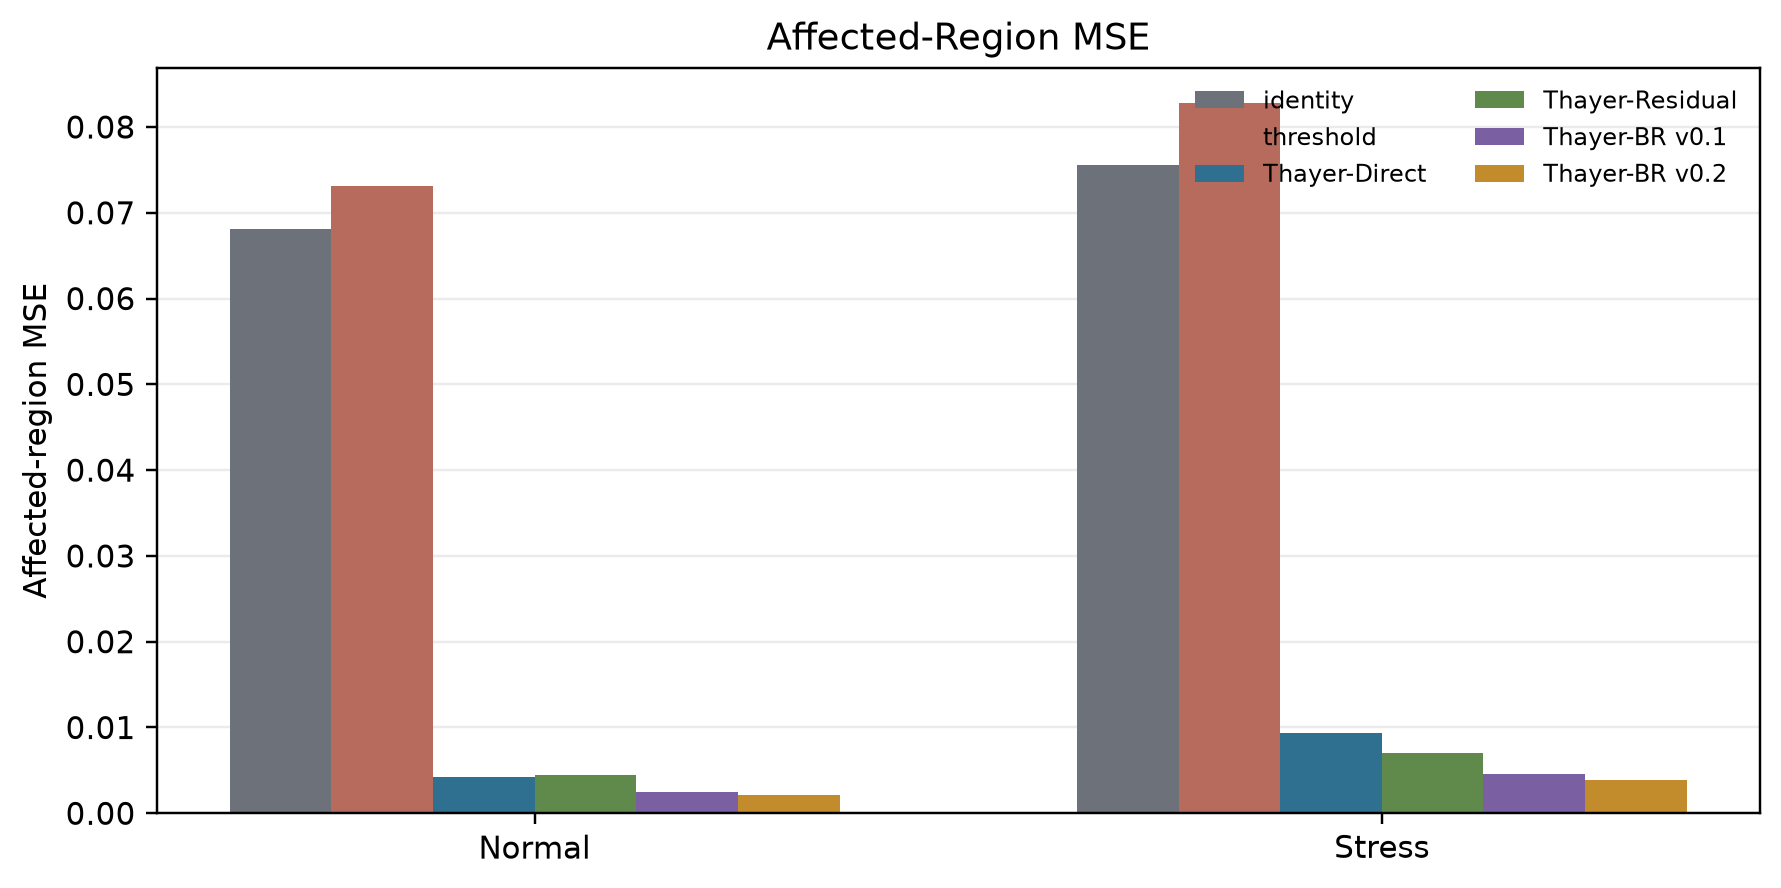
\includegraphics[width=\linewidth]{v02_affected_mse_bar.png}
    \caption{Affected-region MSE for identity, threshold, Thayer-Direct,
    Thayer-Residual, Thayer-BR v0.1, and Thayer-BR v0.2 Moderate.
    Affected-region metrics focus evaluation on the thresholded blend-to-target
    change region. Values are original development results.}
    \label{fig:affected-mse}
\end{figure}

\begin{figure}[t]
    \centering
    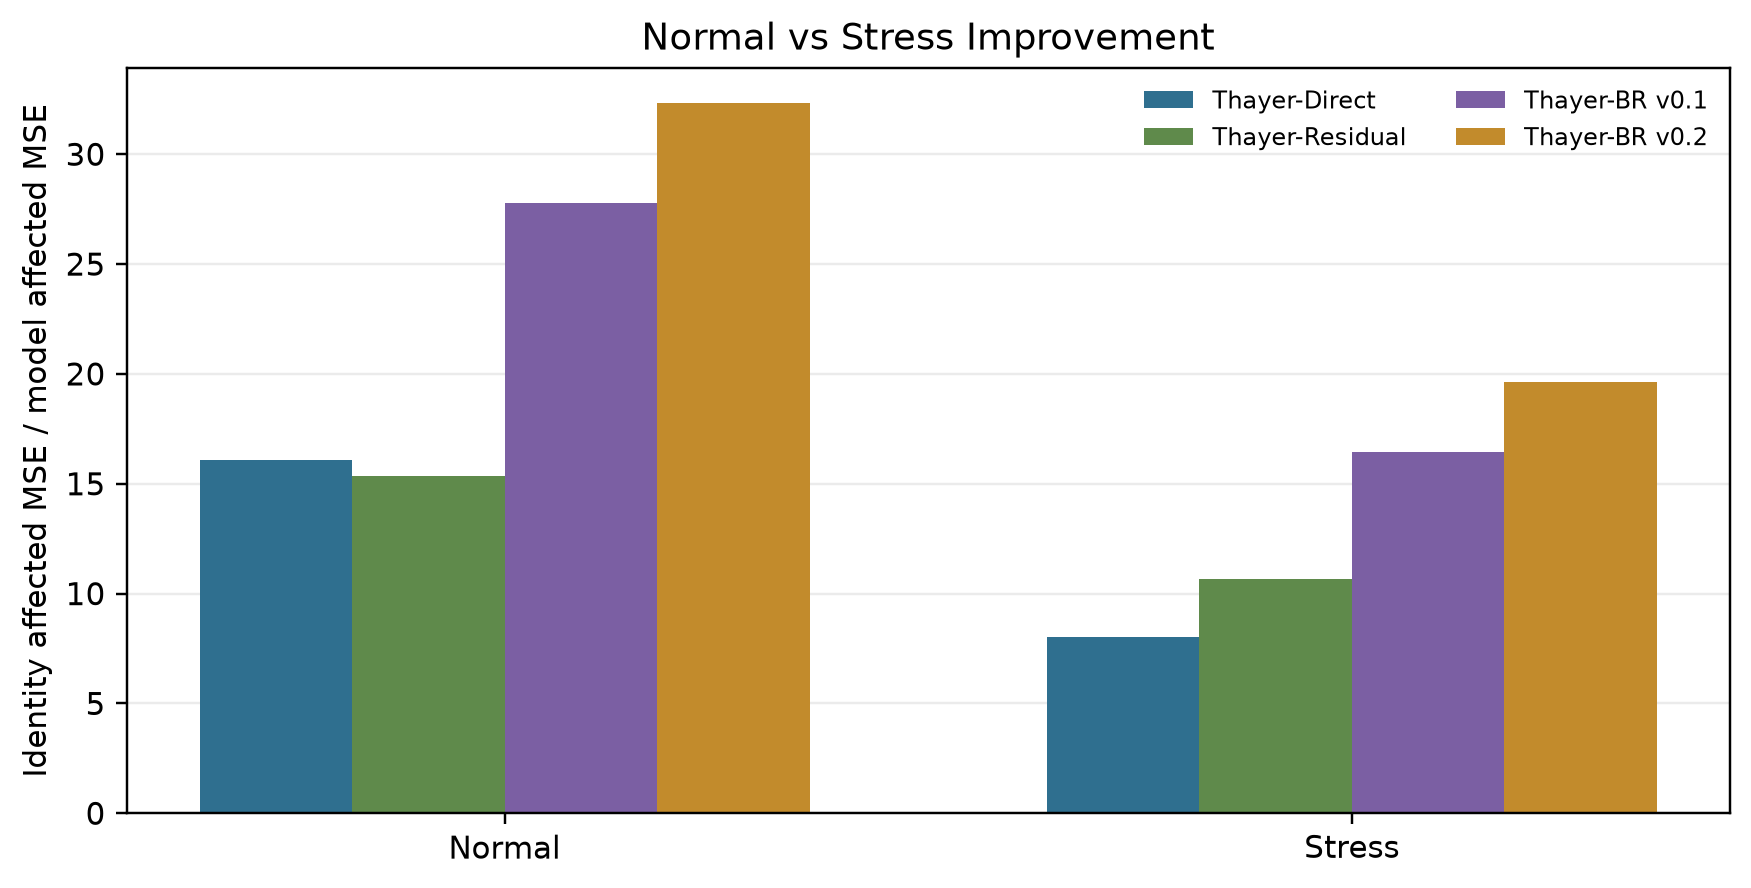
\includegraphics[width=\linewidth]{v02_improvement_ratio.png}
    \caption{Original development improvement ratio versus identity. These
    historical values are retained separately from grouped development results.}
    \label{fig:normal-stress-improvement}
\end{figure}

On the original 1,000-blend comparable normal development evaluation, identity
affected-region MSE is 0.068122. Thayer-Direct reaches 0.004236,
Thayer-Residual reaches 0.004431, Thayer-BR v0.1 reaches 0.002451, and
Thayer-BR v0.2 Moderate reaches 0.002108. This corresponds to about 32.3x
lower affected-region MSE than identity for v0.2 Moderate.

On the hard stress test, identity affected-region MSE is 0.075541.
Thayer-Direct reaches 0.009390, Thayer-Residual reaches 0.007069,
Thayer-BR v0.1 reaches 0.004587, and Thayer-BR v0.2 Moderate reaches 0.003847.
This corresponds to about 19.6x lower affected-region MSE than identity for
v0.2 Moderate.

The source-group-disjoint v0.2 retrain gives 0.00231890 affected MSE on grouped
normal development data (28.8127x lower than identity), 0.00458983 on hard
stress (15.8025x), 0.00872771 on compact-bright stress (9.18304x), and
0.00491680 on high-core-obstruction stress (15.8378x). Worse-than-identity
counts are 0, 3, 2, and 1 out of 1,000, respectively. These grouped values are
the more defensible development estimates, but remain non-final and come from
one training seed.

\begin{figure}[t]
    \centering
    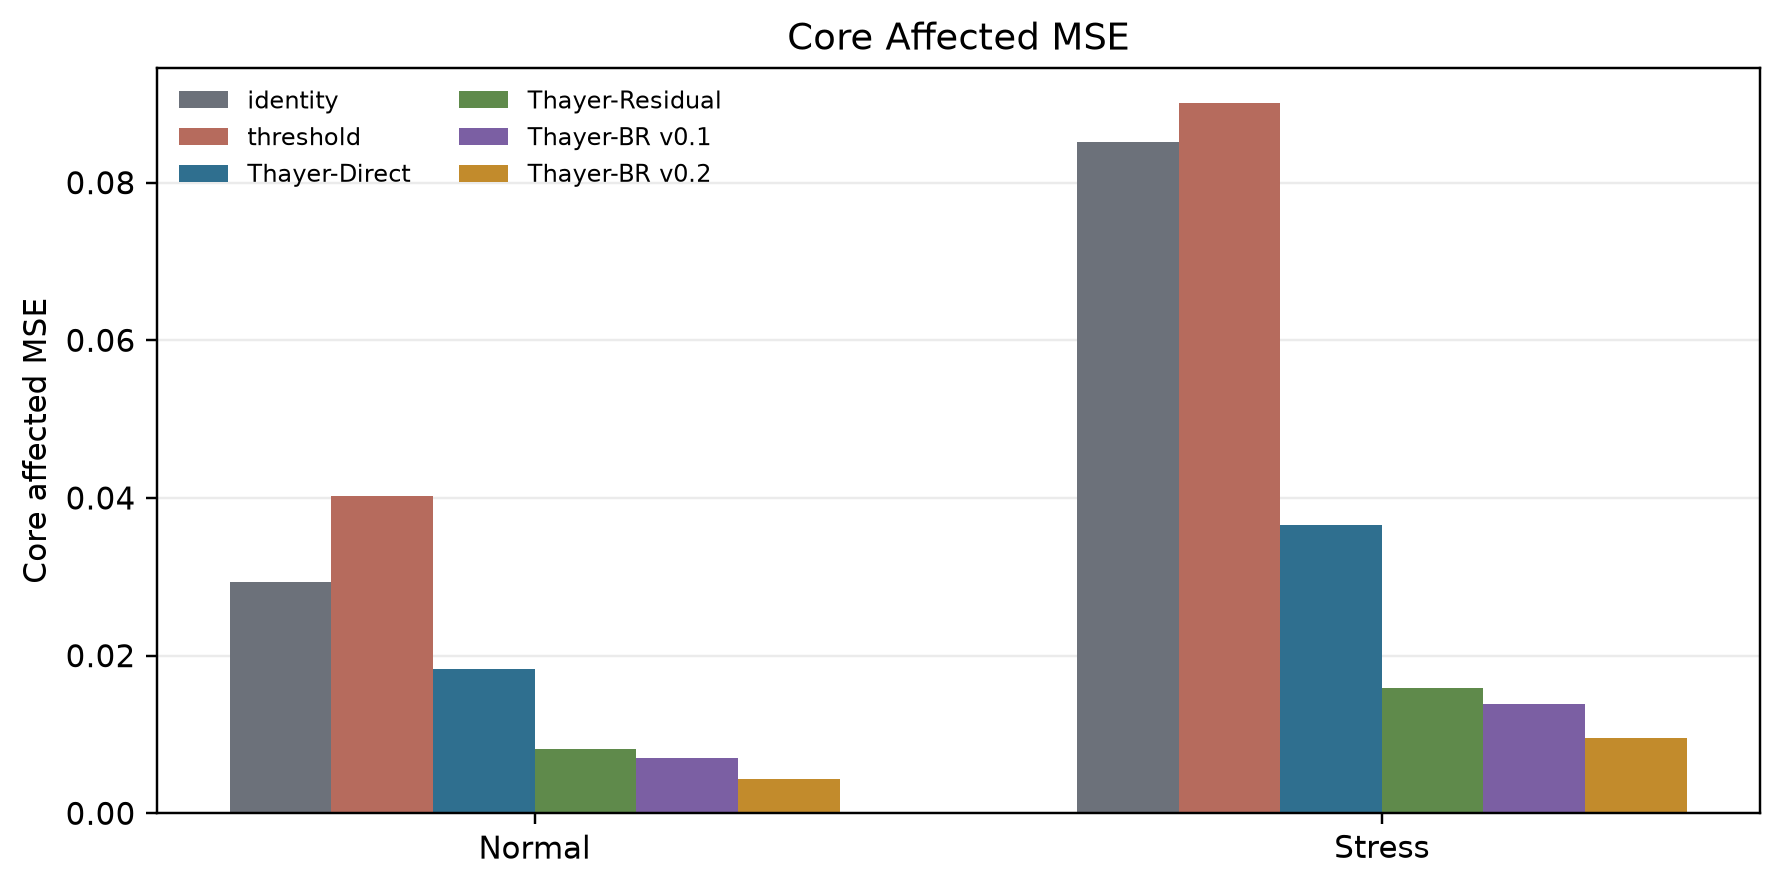
\includegraphics[width=\linewidth]{v02_core_mse.png}
    \caption{Original row-index development core affected MSE comparison.
    Thayer-BR v0.2 Moderate improves stress core affected MSE from 0.013848 for
    Thayer-BR v0.1 to 0.009533.}
    \label{fig:core-mse}
\end{figure}

\begin{figure}[t]
    \centering
    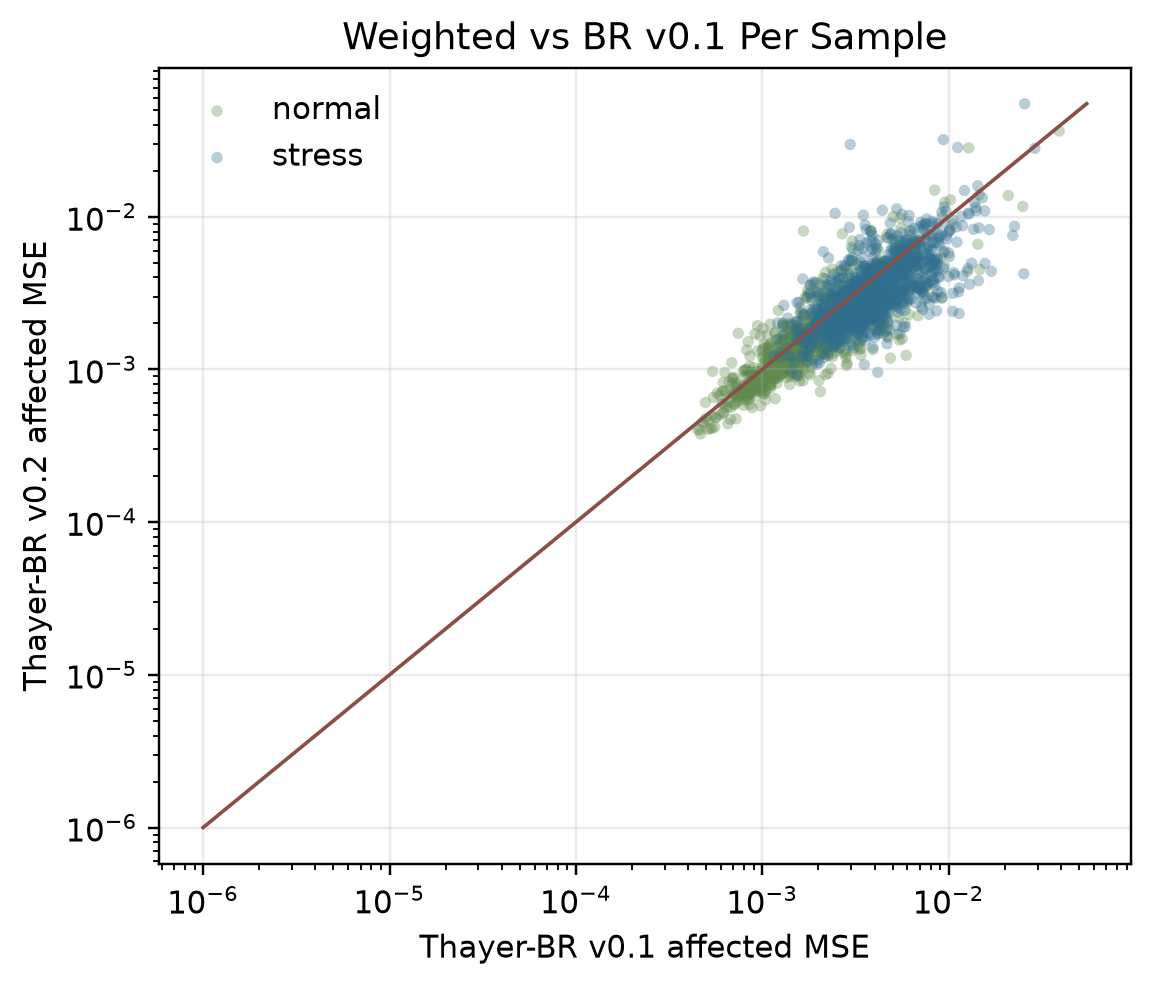
\includegraphics[width=\linewidth]{v02_weighted_vs_v01_scatter.png}
    \caption{Original row-index development per-sample affected-region MSE for
    Thayer-BR v0.2 Moderate versus Thayer-BR v0.1. Points below the parity line
    favor v0.2 Moderate.}
    \label{fig:v02-v01-scatter}
\end{figure}

On the original row-index development suites, compared with Thayer-BR v0.1,
Thayer-BR v0.2 Moderate lowers normal
affected-region MSE by about 14\%, stress affected-region MSE by about 16\%,
and stress core affected MSE by about 31\%. Normal worse-than-identity cases
fall from 1/1000 for v0.1 to 0/1000 for v0.2 Moderate; both models have 0/1000
stress worse-than-identity cases.

\begin{figure}[t]
    \centering
    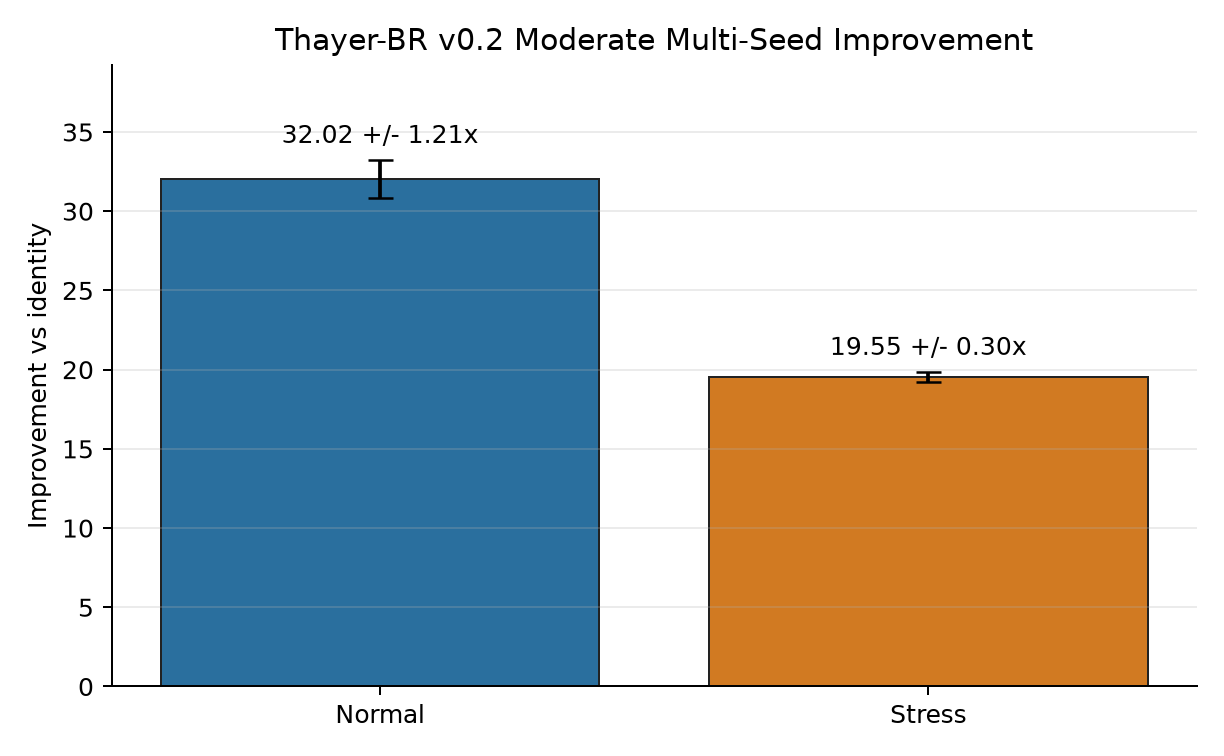
\includegraphics[width=0.75\linewidth]{v02_multiseed_summary.png}
    \caption{Evaluation-seed affected-MSE ratio for the original Thayer-BR v0.2
    Moderate checkpoint. Across
    three normal and three stress evaluation seeds, the model reaches
    32.02 +/- 1.21x normal and 19.55 +/- 0.30x stress. These are not independent
    training seeds.}
    \label{fig:multiseed}
\end{figure}

In the original development ablation, the stronger v0.2 weighting slightly
improves stress core MSE
relative to Moderate, but worsens aggregate normal affected MSE, stress
affected MSE, and stress non-core affected MSE. Moderate weighting is therefore
the best current v0.2 setting.

\begin{figure}[t]
    \centering
    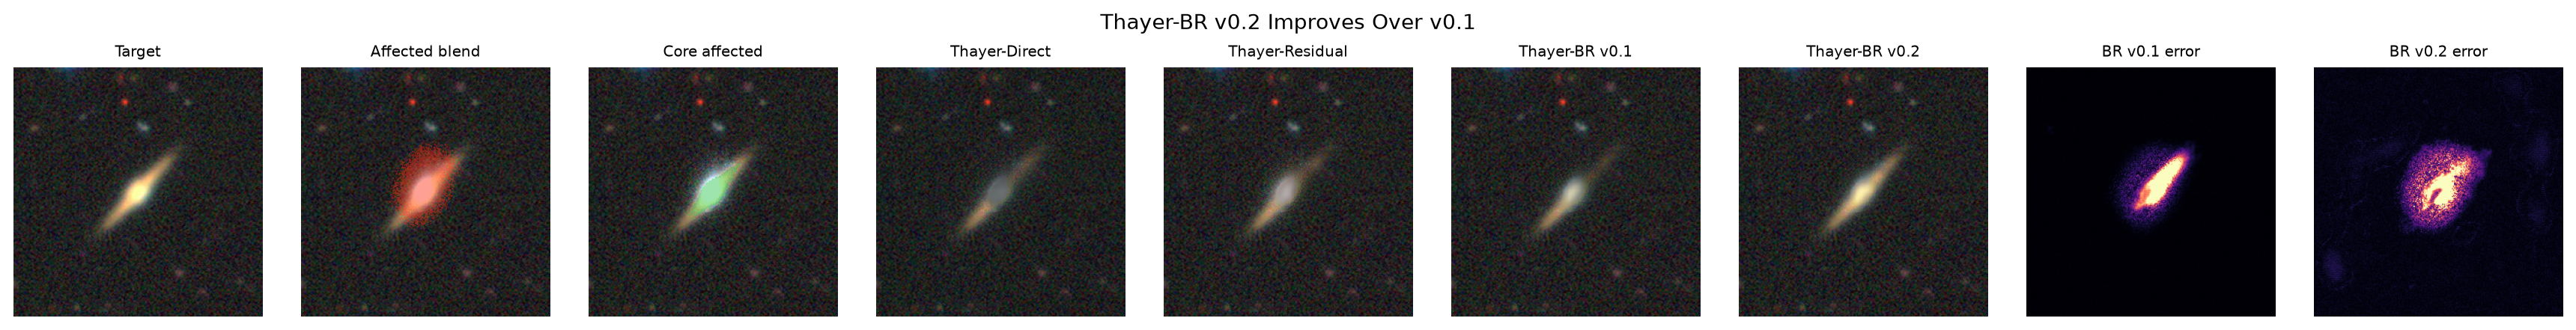
\includegraphics[width=\linewidth]{v02_weighted_improvement_example.png}
    \caption{Qualitative example where Thayer-BR v0.2 Moderate improves over
    Thayer-BR v0.1.}
    \label{fig:v02-success}
\end{figure}

\begin{figure}[t]
    \centering
    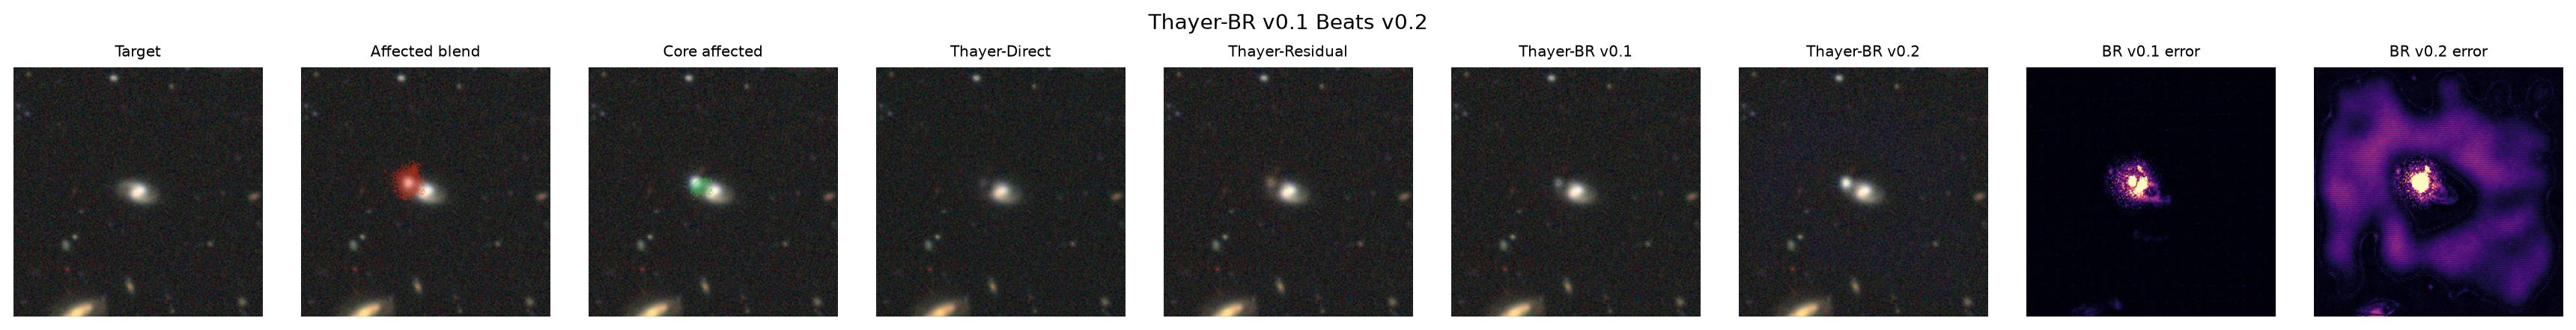
\includegraphics[width=\linewidth]{v02_counterexample.png}
    \caption{Qualitative counterexample where Thayer-BR v0.1 beats
    Thayer-BR v0.2 Moderate on an individual sample. Such cases motivate
    visual-vs-metric diagnostics and limitation figures.}
    \label{fig:v02-counterexample}
\end{figure}


\section{Discussion}
The Thayer-Direct result shows that the controlled synthetic task is learnable:
learned reconstruction substantially improves affected-region error over
identity and threshold baselines. The hard stress test shows that normal
held-out performance is not enough to characterize robustness.

Thayer-Residual helps because the model learns contaminant light to subtract
rather than redrawing the whole target. This can preserve target structure in
regions that are already correct in the blended image. Thayer-BR v0.1 helps
because core overlap and bright/similar-size contaminants are
sampled deliberately during optimization instead of appearing only by chance.

The result should not be overstated. Thayer-Direct and Thayer-Residual still
win on some individual samples. Some failures involve ambiguous overlap,
target-core obstruction, over-smoothing, or lost target detail. Also, high blend
severity is not identical to model difficulty: an obvious contaminant can be
severe but easy to subtract, while a small overlap can be hard if it destroys
central target structure.

The current benchmark remains synthetic. More realistic sky backgrounds, PSF
variation, correlated source environments, and survey-like noise are needed
before making broader astronomical claims.


\section{Conclusion}
Thayer-Net provides a controlled setting for studying compact U-Net models on
synthetic galaxy deblending. Direct reconstruction establishes a strong learned
baseline over identity and threshold methods. Stress testing exposes robustness
loss under harder overlap conditions. Residual prediction improves stress
robustness, balanced hard-case training improves it further, and moderate
affected/core-weighted residual loss gives the strongest current aggregate
result.

Thayer-BR v0.2 Moderate is therefore the current best model for this controlled
synthetic benchmark. The main conclusion is that objective design, training
distribution, and region-aware loss weighting all matter. The next step is to
write up the current result carefully, include counterexamples and audit
figures, preserve exact generated evaluation sets for future audits, and test a
size-normalized held-out benchmark before making stronger claims about
size-invariant or real-sky deblending.


\bibliographystyle{plain}
\bibliography{references}

\end{document}
